\section{Results and Discussion}

\subsection{Low-Level Properties}

Mutational Walk

\begin{figure}
\begin{center}

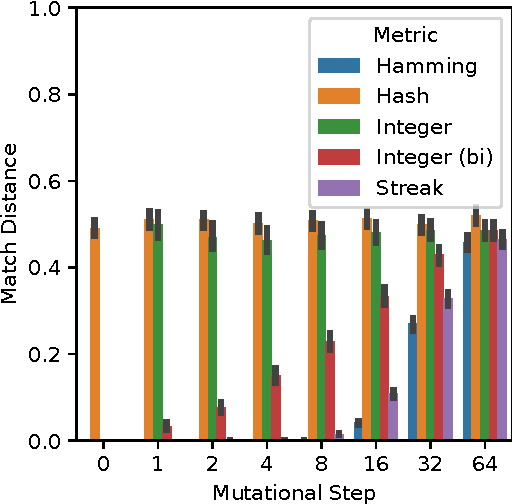
\includegraphics[width=\columnwidth]{{{mutational_walk/bitweight=0.5+seed=1+title=mutational_walk_barplot+_data_hathash_hash=8bf152d87daa9cb7+_script_fullcat_hash=982405ca713eba73+ext=}}}
\caption{
Snapshots of match distance at exponentially increasing steps from identical tags.
Error bars represent 95\% confidence intervals.
}
\label{fig:mutational_walk_barplot}

\end{center}
\end{figure}

\begin{figure*}
\begin{center}

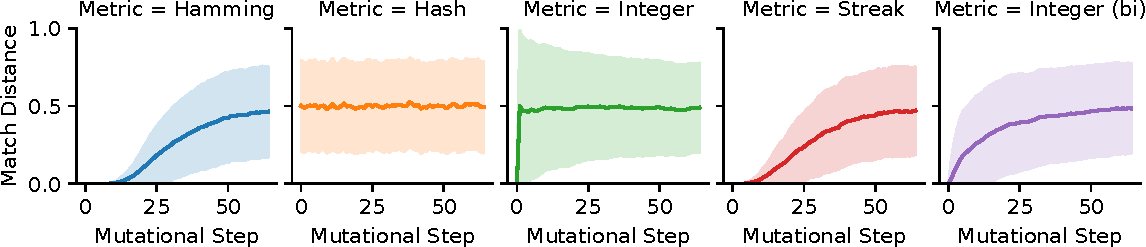
\includegraphics[width=\textwidth]{{{mutational_walk/bitweight=0.5+seed=1+title=mutational_walk_lineplot+_data_hathash_hash=ff15c8831d4f9288+_script_fullcat_hash=c872df869f05035a+ext=}}}
\caption{
TODO
}
\label{fig:mutational_walk_lineplot}

\end{center}
\end{figure*}


Detour Difference

\begin{figure}
\begin{center}

\begin{minipage}{\linewidth}
\begin{subfigure}[b]{\linewidth}
\begin{minipage}{0.5\textwidth}
\begin{center}
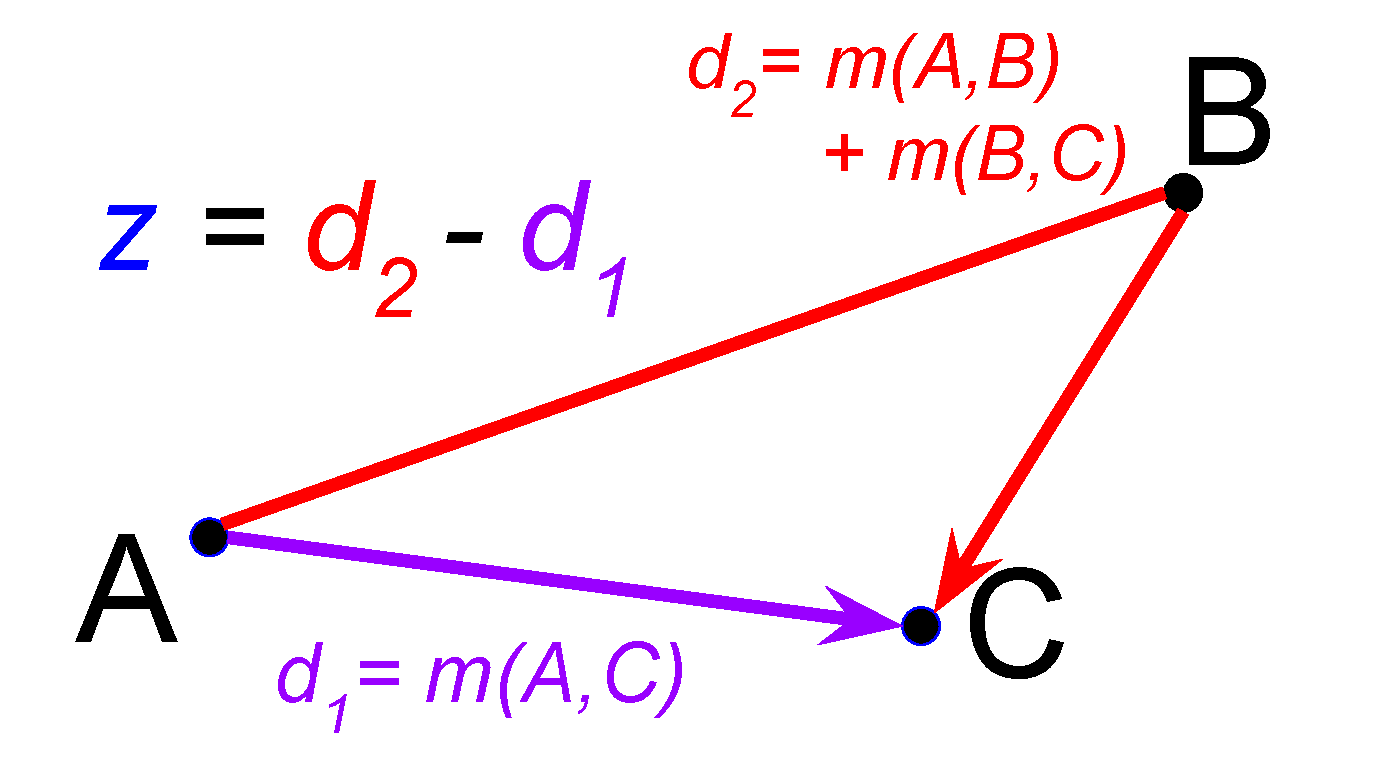
\includegraphics[width=\linewidth,trim=2cm 5cm 2cm 5cm, clip]{detour-difference}
\end{center}
\end{minipage}%
\begin{minipage}{0.5\textwidth}
\caption{
Sampling process used to evaluate detour difference, $z$.
} \label{fig:detour_difference_cartoon}
\end{minipage}
\end{subfigure}
\end{minipage}

\begin{minipage}{\linewidth}
\begin{subfigure}[b]{\linewidth}
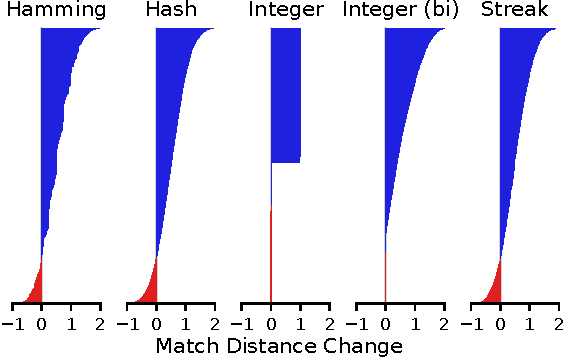
\includegraphics[width=\linewidth]{detour_difference/bitweight=0dot5+seed=1+title=low-triplet-analysis+_data_hathash_hash=6b0749ef97a58721+_script_fullcat_hash=297c4fe09078e17b+ext=}
\caption{
Distributions of detour distance difference for triplets of randomly sampled tags.
Each bar sliver represents an independently sampled observation.
A positive value (colored blue) indicates that total distance increased with the addition of an intermediate stop.
A value of exactly 0 indicates an intermediate stop had no effect on total distance.
A negative value (colored red) indicates violation of the triangle inequality: taking an intermediate stop reduced the total distance travelled.
} \label{fig:detour_difference_distribution}

\end{subfigure}
\end{minipage}

\caption{
Detour difference of tag-matching metrics.
}
\label{fig:detour_difference}

\end{center}
\end{figure}


most extreme out of 5000 randomly generated triplets

Hamming
-0.7554609929831894

Streak
-0.9114630155495477

Hash

-0.9316840054175641

Integer (bi)
-0.0005741139882278224

Integer
-0.00029025424747706693

% \subsection{Expressiveness}
%
% best fitness after lots of generations, one link per vs irregular
% \begin{figure*}[!htbp]
% \begin{center}
%   \begin{subfigure}[b]{0.5\linewidth}
%     \includegraphics[width=\linewidth]{{{bitweight=0.5+experiment=mid-flex-match+fit-fun=ranked+viz=fitness-max+_data_hathash_hash=b681f20513e727bb+_script_fullcat_hash=eb40b1f6164b4595+ext=}}}
%     \caption{high mutation rate}
%     \label{fig:TODO}
%   \end{subfigure}
%   \begin{subfigure}[b]{0.5\linewidth}
%     TODO
%     \caption{low mutation rate}
%     \label{fig:TODO}
%   \end{subfigure}
% \caption{
% mean bar plot
% }
% \label{fig:TODO}
% \end{center}
% \end{figure*}
%
% best fitness after lots of generations, one link per vs irregular
% \begin{figure*}[!htbp]
% \begin{center}
%   \begin{subfigure}[b]{0.5\linewidth}
%     \includegraphics[width=\linewidth]{{{bitweight=0.5+experiment=mid-flex-match+fit-fun=ranked+viz=fitness-mean-max+_data_hathash_hash=b681f20513e727bb+_script_fullcat_hash=4bad04320cec1da1+ext=}}}
%     \caption{high mutation rate}
%     \label{fig:TODO}
%   \end{subfigure}
%   \begin{subfigure}[b]{0.5\linewidth}
%     TODO
%     \caption{low mutation rate}
%     \label{fig:TODO}
%   \end{subfigure}
% \caption{
% max bar plot
% }
% \label{fig:TODO}
% \end{center}
% \end{figure*}
%
%
% \begin{figure*}[!htbp]
% \begin{center}
%   \begin{subfigure}[b]{0.5\linewidth}
%     \includegraphics[width=\linewidth]{{{bitweight=0.5+experiment=mid-flex-match+fit-fun=ranked+viz=fitness-line+_data_hathash_hash=b681f20513e727bb+_script_fullcat_hash=97943b1863adc763+ext=}}}
%     \caption{high mutation rate}
%     \label{fig:TODO}
%   \end{subfigure}
%   \begin{subfigure}[b]{0.5\linewidth}
%     TODO
%     \caption{low mutation rate}
%     \label{fig:TODO}
%   \end{subfigure}
% \caption{
% max line plot
% }
% \label{fig:TODO}
% \end{center}
% \end{figure*}
%
% \begin{figure*}[!htbp]
% \begin{center}
%   \begin{subfigure}[b]{0.5\linewidth}
%     \includegraphics[width=\linewidth]{{{bitweight=0.5+experiment=mid-flex-match+fit-fun=ranked+viz=fitness-mean-line+_data_hathash_hash=b681f20513e727bb+_script_fullcat_hash=4bad04320cec1da1+ext=}}}
%     \caption{high mutation rate}
%     \label{fig:TODO}
%   \end{subfigure}
%   \begin{subfigure}[b]{0.5\linewidth}
%     TODO
%     \caption{low mutation rate}
%     \label{fig:TODO}
%   \end{subfigure}
% \caption{
% mean line plot
% }
% \label{fig:TODO}
% \end{center}
% \end{figure*}
%
% \subsection{Evolutionary Speed}
%
% \begin{figure*}[!htbp]
% \begin{center}
%   \begin{subfigure}[b]{0.5\linewidth}
%     \includegraphics[width=\linewidth]{{{bitweight=0.5+experiment=mid-flex-match+fit-fun=ranked+viz=fitness-best+_data_hathash_hash=b681f20513e727bb+_script_fullcat_hash=dbb1d5f8d167dcfb+ext=}}}
%     \caption{high mutation rate}
%     \label{fig:TODO}
%   \end{subfigure}
%   \begin{subfigure}[b]{0.5\linewidth}
%     TODO
%     \caption{low mutation rate}
%     \label{fig:TODO}
%   \end{subfigure}
% \caption{
% TODO focus on start of evolution, should this be a bar plot of updates until first perfect soluiton?
% }
% \label{fig:TODO}
% \end{center}
% \end{figure*}
%
%
% fitness by generation, one link per vs irregular
%
% 16 vs 32 targets
%
% \subsection{Neutrality}
%
% \begin{figure*}[!htbp]
% \begin{center}
%   \begin{subfigure}[b]{0.5\linewidth}
%     \includegraphics[width=\linewidth]{{{bitweight=0.5+experiment=mid-flex-match+fit-fun=ranked+viz=neutrality-ancestry-line+_data_hathash_hash=c232a31962b449a7+_script_fullcat_hash=2890a55353ee6039+ext=}}}
%     \caption{high mutation rate}
%     \label{fig:TODO}
%   \end{subfigure}
%   \begin{subfigure}[b]{0.5\linewidth}
%     TODO
%     \caption{low mutation rate}
%     \label{fig:TODO}
%   \end{subfigure}
% \caption{
% Eventually should be a bar plot
% }
% \label{fig:TODO}
% \end{center}
% \end{figure*}
%
% \begin{figure*}[!htbp]
% \begin{center}
%   \begin{subfigure}[b]{0.5\linewidth}
%     \includegraphics[width=\linewidth]{{{bitweight=0.5+experiment=mid-flex-match+fit-fun=ranked+viz=robustness-bar+_data_hathash_hash=4fe7e4700966f117+_script_fullcat_hash=6ea9986118610f4a+ext=}}}
%     \caption{high mutation rate}
%     \label{fig:TODO}
%   \end{subfigure}
%   \begin{subfigure}[b]{0.5\linewidth}
%     TODO
%     \caption{low mutation rate}
%     \label{fig:TODO}
%   \end{subfigure}
% \caption{
% Mutations until first phenotypic change
% }
% \label{fig:TODO}
% \end{center}
% \end{figure*}
%
%
% mutational walk
%
% number of mutations to first phenotypic change
%
% long-term genetic distance
% (e.g., over 16, 64, 256, 1024 generations)
%
% \subsection{Modularity}
%
% \begin{figure*}[!htbp]
% \begin{center}
% \begin{subfigure}[b]{0.5\linewidth}
%   \includegraphics[width=\linewidth]{{{bitweight=0.5+experiment=mid-flex-match+fit-fun=ranked+viz=mutation-modularity-violin+_data_hathash_hash=01e5cfbd6360506b+_script_fullcat_hash=6abaf7fcf2beda8b+ext=}}}
%   \caption{violin plot}
%   \label{fig:TODO}
% \end{subfigure}
% \begin{subfigure}[b]{0.5\linewidth}
%   \includegraphics[width=\linewidth]{{{bitweight=0.5+experiment=mid-flex-match+fit-fun=ranked+viz=mutation-modularity-bar+_data_hathash_hash=01e5cfbd6360506b+_script_fullcat_hash=6abaf7fcf2beda8b+ext=}}}
%   \caption{bar graph}
%   \label{fig:TODO}
% \end{subfigure}
% \caption{
% Mean
% }
% \label{fig:modularity}
% \end{center}
% \end{figure*}


\subsection{Promiscuity}

best fitness to try to evolve a hub

REGULATION

ideas: bitweight, wildcards

if first bit set, divide match score by two
